%%for slideshow
\documentclass[ignorenonframetext]{beamer} %add option 'draft' for quicker compilation
\usepackage{amsmath,amssymb,multirow}
\newcommand{\slides}{1}
%this only compiles frames with [label=current]
%\includeonlyframes{current} 
 
%for handouts
%\documentclass[a4paper,12pt]{article}
%\usepackage{beamerarticle}
%\newcommand{\slides}{0}

\mode<presentation>{
% for theme info see:
% http://www.ctan.org/tex-archive/macros/latex/contrib/beamer/doc/beameruserguide.pdf
\usetheme{default}
  \setbeamercovered{transparent}
  %Add university logo
  %\pgfdeclareimage[height=1cm]{university-logo}{logo}
  %\logo{\pgfuseimage{university-logo}}
  % If you wish to uncover everything in a step-wise fashion, uncomment
  % the following command:
%  \beamerdefaultoverlayspecification{<+->}
	\newcommand{\tcr}{\textcolor{red}}
}
\mode<article>{
  \usepackage{fullpage}
	\newcommand{\tcr}{\textcolor{black}}
  \renewcommand{\baselinestretch}{1.0}
  \oddsidemargin -1.5cm \evensidemargin -1.5in
  \topmargin=-1.5cm \headheight=0pt
  \headsep 0pt \textwidth=19cm
  \textheight=27cm \columnsep 10pt \columnseprule 0pt \parindent 0pt
  \parskip 0.0pt
  \usepackage{tweaklist}
  \renewcommand{\itemhook}{
    \setlength{\topsep}{-0pt}
    \setlength{\itemsep}{-0pt}
    \setlength{\parsep}{-0pt}
  }
  \renewcommand{\enumhook}{
    \setlength{\topsep}{-0pt}
    \setlength{\itemsep}{-0pt}
    \setlength{\parsep}{-0pt}
  }
}

\usepackage[english]{babel}
\usepackage[latin1]{inputenc}
\usepackage{times}
\usepackage[T1]{fontenc}
\usepackage{graphics,graphicx,fancyhdr,color,amsmath,url,enumerate,alltt}
\usepackage{epsf}
\usepackage{ifthen}


\newcommand{\bc}{\begin{center}}
\newcommand{\ec}{\end{center}}
\newcommand{\bn}{\begin{enumerate}}
\newcommand{\en}{\end{enumerate}}
\newcommand{\bi}{\begin{itemize}}
\newcommand{\ei}{\end{itemize}}
\newcommand{\be}{\begin{eqnarray}}
\newcommand{\ee}{\end{eqnarray}}
\newcommand{\bes}{\begin{eqnarray*}}
\newcommand{\ees}{\end{eqnarray*}}
\newcommand{\expect}[1]{\mathbb{E}\left[ #1 \right]}


\title[Smoothing over complex regions]{Two new approaches to smoothing over complex regions}

\author[Miller]{David Lawrence Miller}

\institute{Mathematical Sciences\\University of Bath}

\date[23-25 June 2009] {Modelling complex environmental spatial and temporal data, Bath}
%\date[July 2009] {useR! 2009, Rennes}
% - Either use conference name or its abbreviation.
% - Not really informative to the audience, more for people (including
%   yourself) who are reading the slides online

% Delete this, if you do not want the table of contents to pop up at
% the beginning of each subsection:
\mode<presentation> {
%    \AtBeginSubsection[]
    \AtBeginSection[]
    {
    \begin{frame}<beamer>
        \frametitle{Outline}
        %\tableofcontents[currentsection,currentsubsection]
        \tableofcontents[currentsection]
    \end{frame}
    }
}
\begin{document}

\begin{frame}
  \titlepage
\end{frame}

\mode<article>{
\maketitle
}

\mode<presentation> {
\begin{frame}
  \frametitle{Outline}
  \tableofcontents %[pausesections]
  % You might wish to add the option [pausesections]
\end{frame}
}

\section{Smoothing over complex regions}

\subsection{Intro}

\begin{frame}
	\frametitle{Smoothing in 2 dimensions}
       \bi
         \item Have some geographical region and wish to find out something about the biological population in it. 
         \item Response is eg. animal distribution, wish to predict based on $(x,y)$ and other covariates eg. habitat, size, sex, etc.
         \item This problem is relatively easy if the domain is simple.
       \ei
       \bc
         \includegraphics[width=2.5in]{figs/peninsula}
       \ec
\end{frame}

\begin{frame}
	\frametitle{Smoothing with penalties}
      \bi
         \item Objective function takes the form:
      \ei
      \bc
      \begin{equation*}
      \sum_{i=1}^n (z_i-f(x_i,y_i;\theta))^2 + \lambda \int_\Omega Pf(x,y;\theta)d\Omega
      \end{equation*}
      \ec
      \bi
         \item $f$ is the function you want to estimate, made up of some combination of basis functions.
         \item $P$ is some squared derivative penalty operator, usually $P=(\frac{\partial^2}{\partial x^2}+\frac{\partial^2}{\partial y^2})^2$.
         \item This can be generalized to an additive model or GAM.
      \ei
\end{frame}

\begin{frame}
	\frametitle{Smoothing over complex domains}
       \bi
         \item Smoothing of complex domains makes this a lot more difficult.
         \item Problem of leakage.
         \item Euclidean distance doesn't always make sense.
         \item Models need to incorporate information about the intrinsic structure of the domain.
       \ei
       \bc\begin{tabular}{@{}cc}
          & \\
          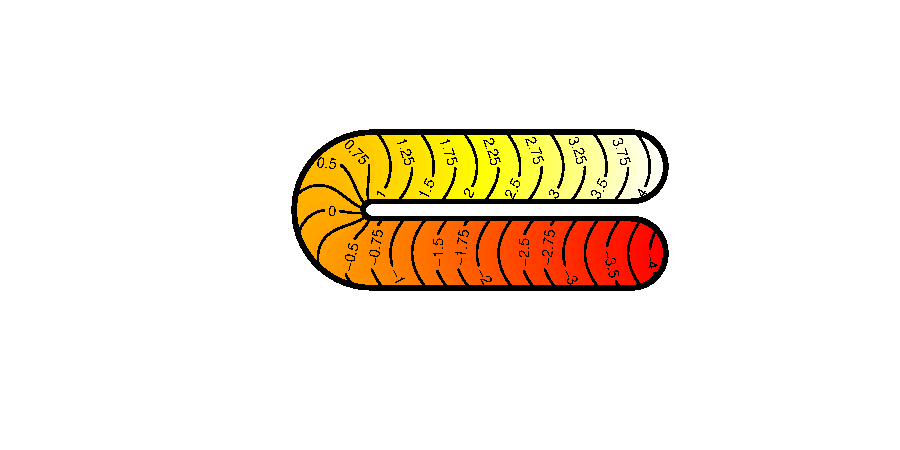
\includegraphics[width=2in, trim=1in 1in 1in 1in]{figs/ramsayhorseshoe} & 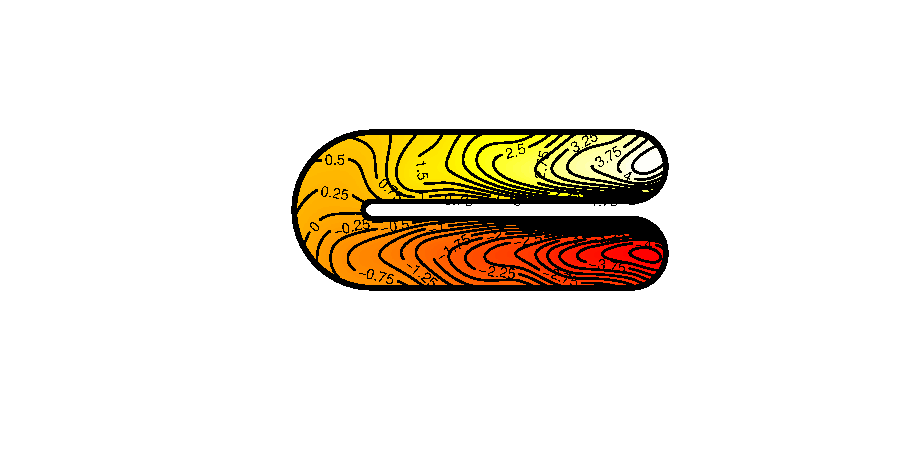
\includegraphics[width=2in, trim=1in 1in 1in 1in]{figs/leakageexample}\\
          (modified) Ramsay test function & Thin plate spline fit\\
       \end{tabular}\ec
\end{frame}

\subsection{Solutions}

\begin{frame}
	\frametitle{Possible solutions to leakage problems}
       \bi
         \item FELSPLINE (Ramsay, (2002).)
         \item Within-area distance (Wang and Ranalli, (2007).)
         \item Soap film smoothers (Wood \emph{et al.} (2008).) 
         \item Domain morphing (Eilers (2006).)
        \ei
\end{frame}

\begin{frame}
	\frametitle{Why morph the domain?}
      \bi
         \item Takes into account within-area distance.
         \item Gives a known domain that is easier to smooth over.
         \item Potentially less computationally intensive. 
      \ei
      \bc
         \textbf{However:}
      \ec
      \bi
         \item Don't maintain isotropy - distribution of points odd.
         \item Not clear what this does to the smoothness penalty.
      \ei
      \bc
         \includegraphics[height=1in]{figs/matlab-test-3}
      \ec
\end{frame}


\section{Domain morphing with the Schwarz-Christoffel transform}

\subsection{Details}

\begin{frame}
	\frametitle{The Schwarz-Christoffel transform}
       \bi
         \item Take a polygon in some domain $W$ and morph it to a new domain $W^*$.
         \item Do this by starting at the new domain and working back to the polygon.
         %\item Example: add extra edges to a rectangle and then alter angles.
         \item Can draw a polygonal bounding box around some arbitrary shape.
        \ei
        \bc
              \includegraphics[height=1in]{figs/mappingdia}
       \ec
\end{frame}


\begin{frame}
	\frametitle{Schwarz-Christoffel algorithm}
       \bi
         \item Start with a rectangle.
         \item Add vertices.
         \item Iteratively deform by changing angles.
         \item Continue until the new shape is identical to the polygon.
         \item We then have a function for the mapping, $\varphi(x,y)$.
         \item $\varphi(x,y)$ is a conformal mapping.
        \ei 
      \bc
         \includegraphics[height=1in]{figs/matlab-test-2}
      \ec
\end{frame}

\subsection{Simulation Results}

\begin{frame}
	\frametitle{The mapping}
      \bi
         \item Use a bounding box around the horseshoe.
      \ei
      \bc
         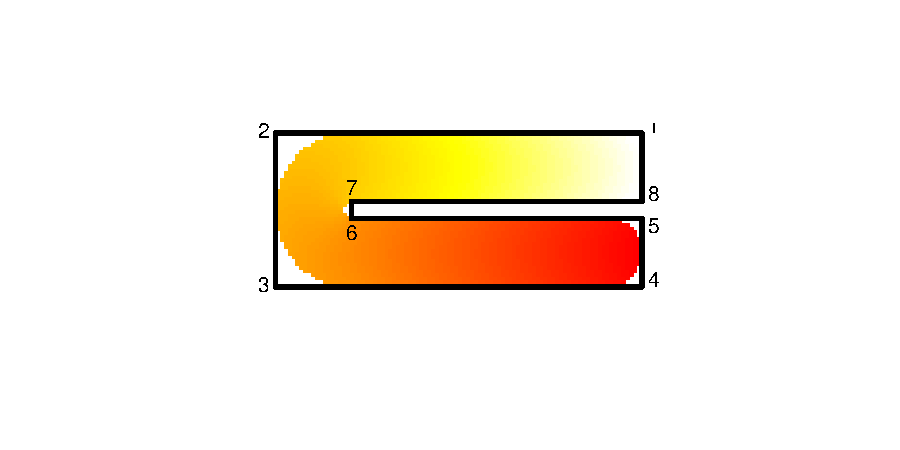
\includegraphics[height=0.75in, trim=1in 1in 1in 0.75in]{figs/hswithboundingbox} 
      \ec
      \bi
         \item Morphing the horseshoe shape still gives a slightly odd domain however, we are still doing better than before.
      \ei
      \bc\begin{tabular}{@{}cc}
          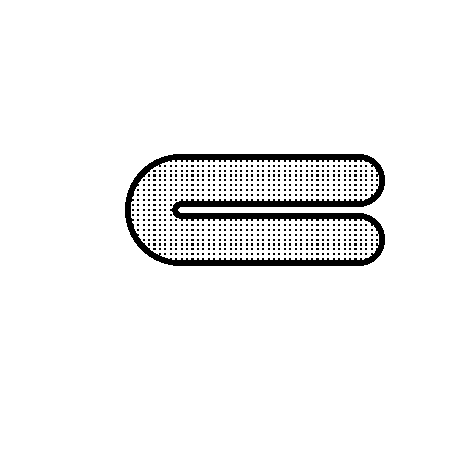
\includegraphics[height=0.75in, trim=1in 1in 0in 0.75in]{figs/hsgridmapping-1} \\ 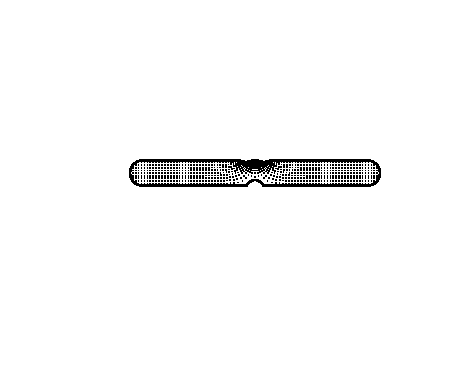
\includegraphics[width=2in, trim=0in 0in 0in 0in]{figs/hsgridmapping-2} \\
       \end{tabular}\ec
\end{frame}

\begin{frame}
	\frametitle{Results}
       \bi
         \item Fit using both thin plate regression splines and P-splines with a comparison to the soap film (current best.) 
         \item MSE used to compare over a grid of predicition points.
         \item Transformation method does well on the horseshoe.
        \ei
       \bc\begin{tabular}{@{}cc}
          \includegraphics[width=2.5in]{figs/tensorproduct} & \includegraphics[width=1in]{figs/tprs}\\
          Tensor product & Thin plate\\
       \end{tabular}\ec
\end{frame}


\begin{frame}
	\frametitle{Horseshoe plots}
            \centering
            % trim order l b r t
          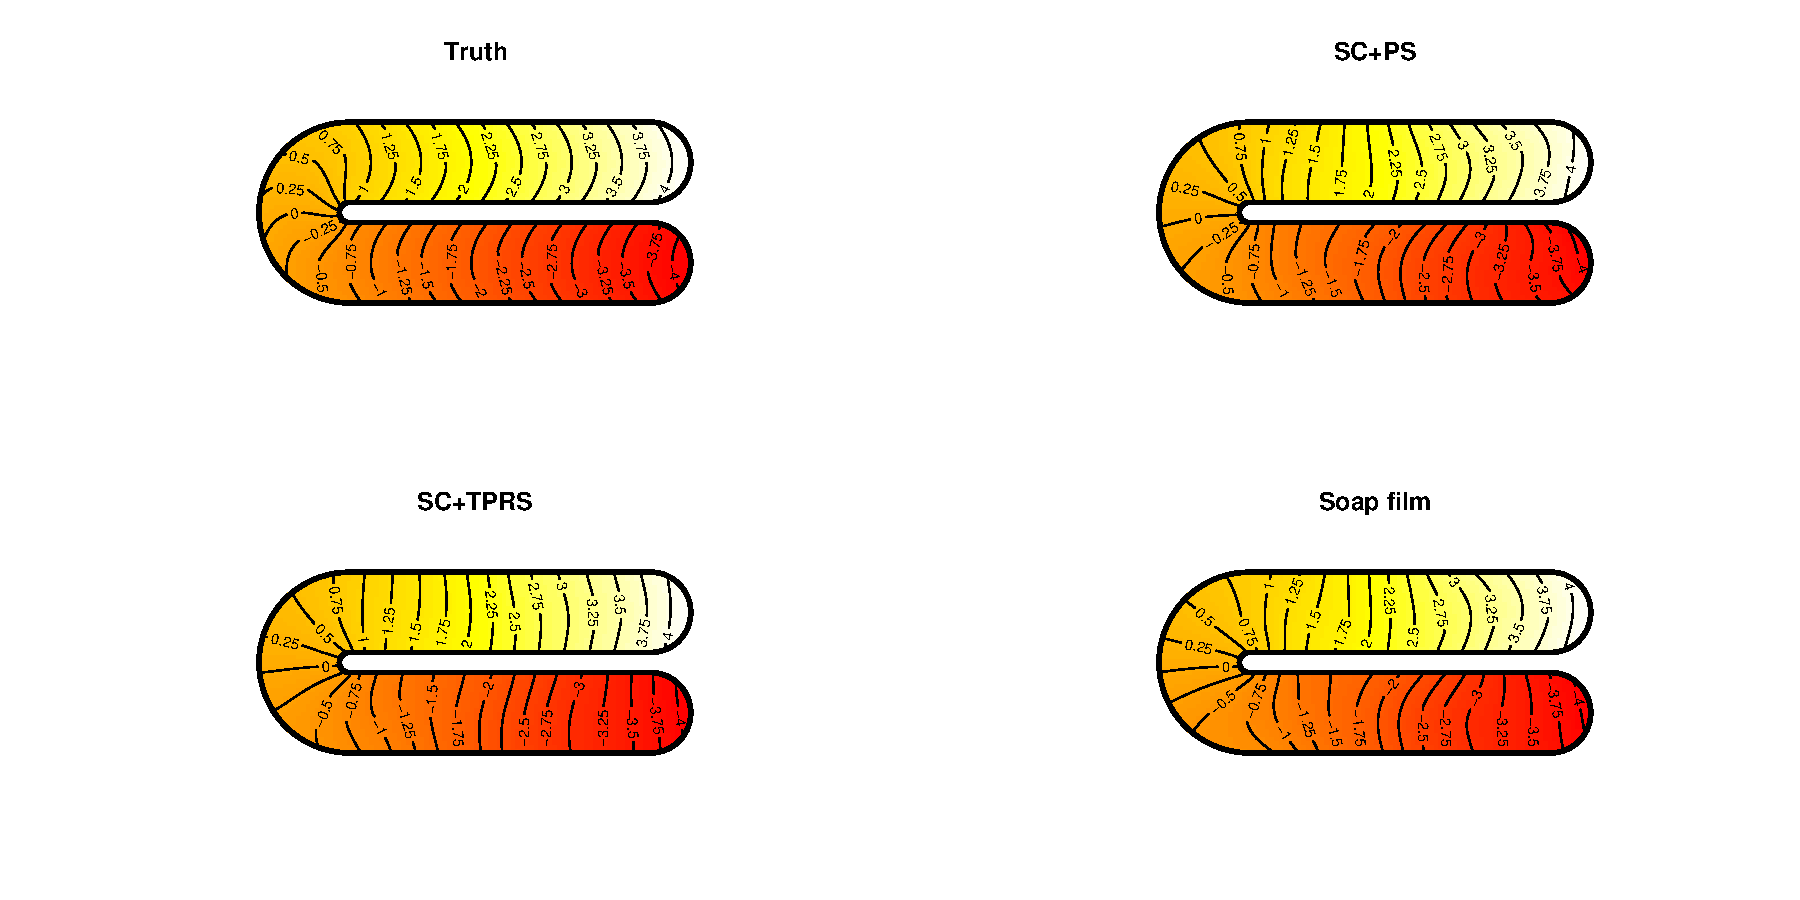
\includegraphics[width=4in,trim=2in 1in 2in 0.5in]{figs/compsmooth}
\end{frame}

\begin{frame}
	\frametitle{Why does it do well?}
       \bi
         \item Looking at line plots, we can see the difference in gradient.
         \item SC method seems to approximate the gradient better.
       \ei
       \bc\begin{tabular}{c c}
            \centering
            % trim order l b r t
          \includegraphics[width=1in, trim=1in 0.75in 0.5in 0.5in]{figs/horseshoecentreline-1} & 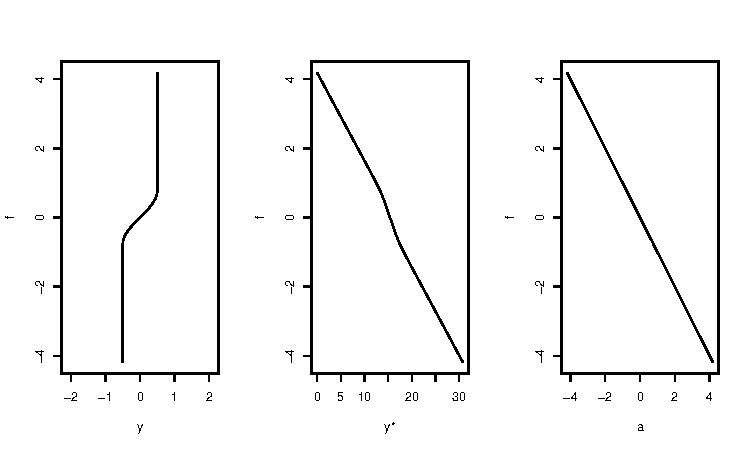
\includegraphics[width=2.5in]{figs/centrelinelineplots}\\
       \end{tabular}\ec
\end{frame}


\begin{frame}
	\frametitle{Problems}
       \bi
         \item Implementation is Matlab+R.
         \item Problems with more realistic situations:
         \bi
         \item Weird artifacts.
         \item Arbitrary selection of vertices.
         \item Morphing of domain appears to cause features to be smoothed over.
         \ei
        \ei
\end{frame}

\begin{frame}
	\frametitle{A more realistic domain}
            \centering
              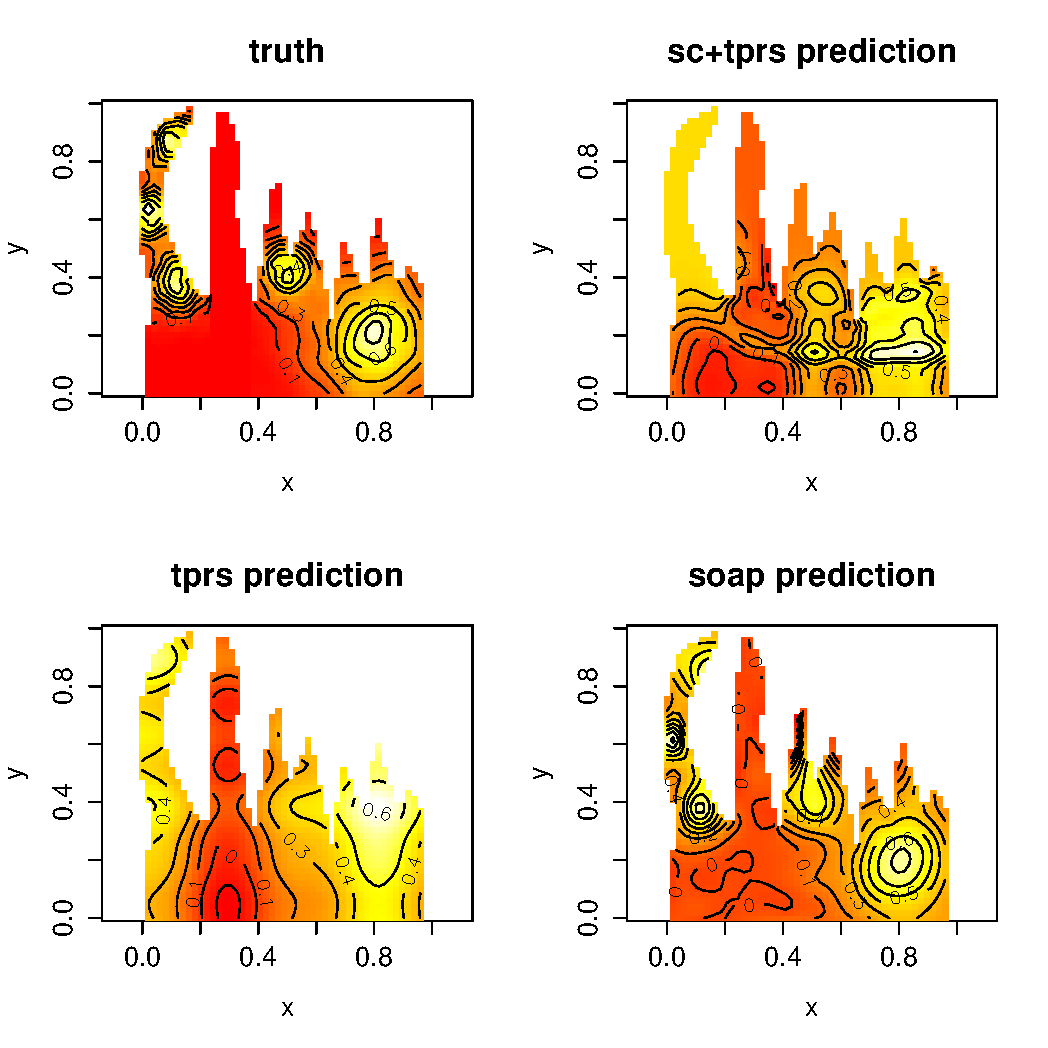
\includegraphics[width=3in]{figs/wigglytop2-real}\\
\end{frame}



\section{Multidimensional Scaling}

\subsection{Details}

\begin{frame}
	\frametitle{Multidimensional scaling and within-area distances}
       \bi
         \item Idea: use MDS to to arrange points in the domain according to their ``within-domain distance.''
         \item First need to find the within area distances.
         \item Can then smooth over the new points.

        \ei
\end{frame}

\begin{frame}
	\frametitle{Multidimensional scaling refresher}
       \bi
         \item Double centre matrix of between point distances, $D$, (subtract row and column means) then find $DD^T$.
         \item Finds a configuration of points such that \item Euclidean distance between points in new arrangement is approximately the same as distance in the domain.
         \item Prediction outside the original data is fine.
         \item Already implemented in \textsf{R} by \texttt{cmdscale}.
        \ei
            \centering
            % this is just generated from wt2-test.R
              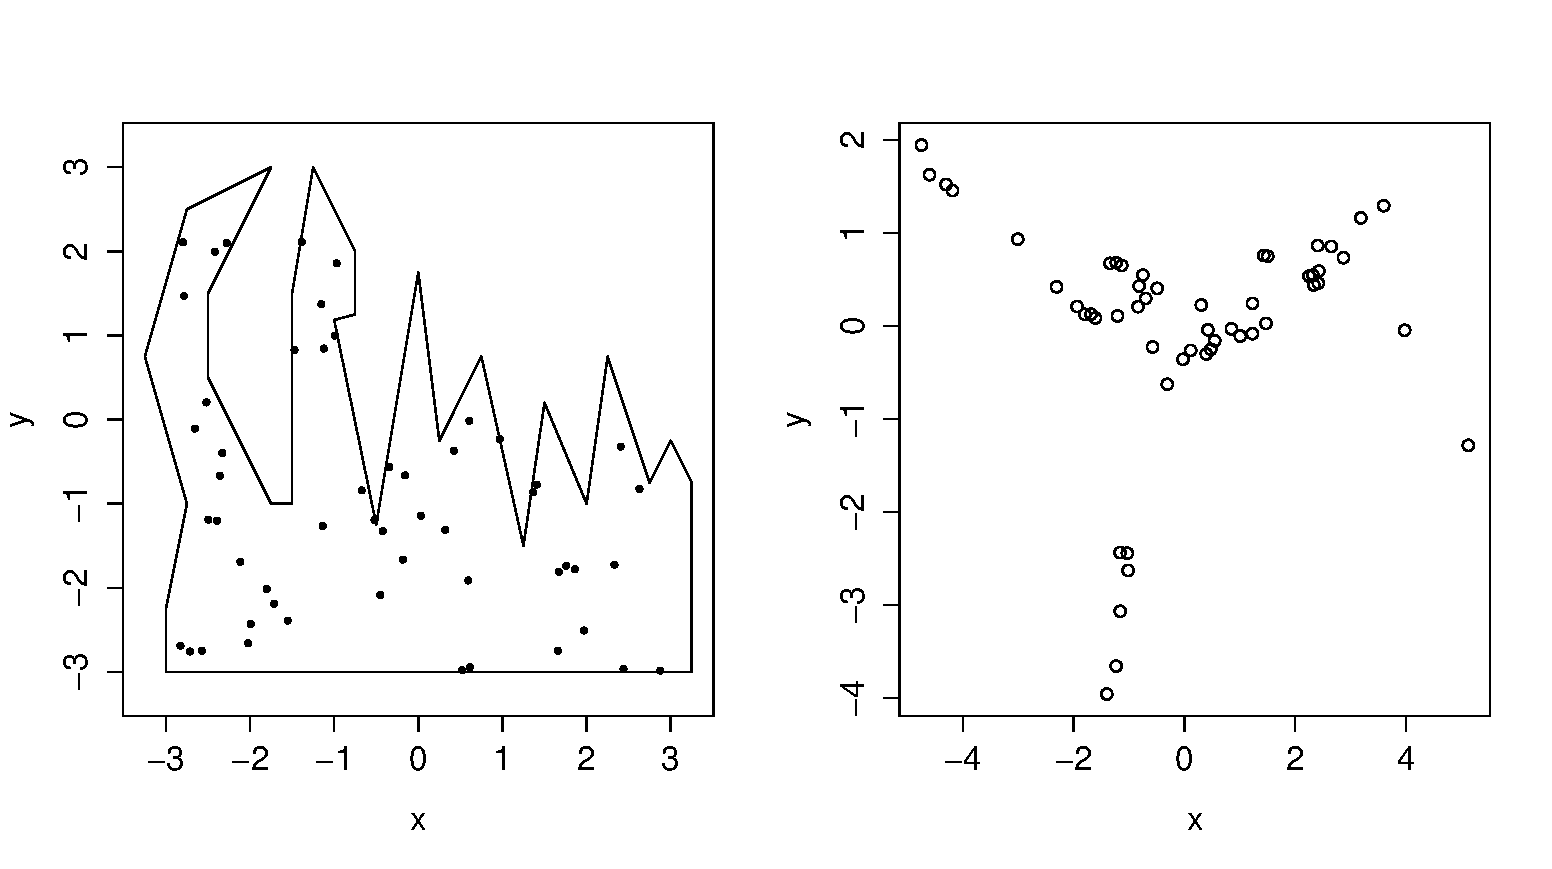
\includegraphics[width=3in]{figs/wt2-pco-example.pdf}\\
        
\end{frame}

\begin{frame}
	\frametitle{Finding within-area distances}
       \bi
         \item Use a new algorithm to find the within area distances.
        \ei
            \centering
              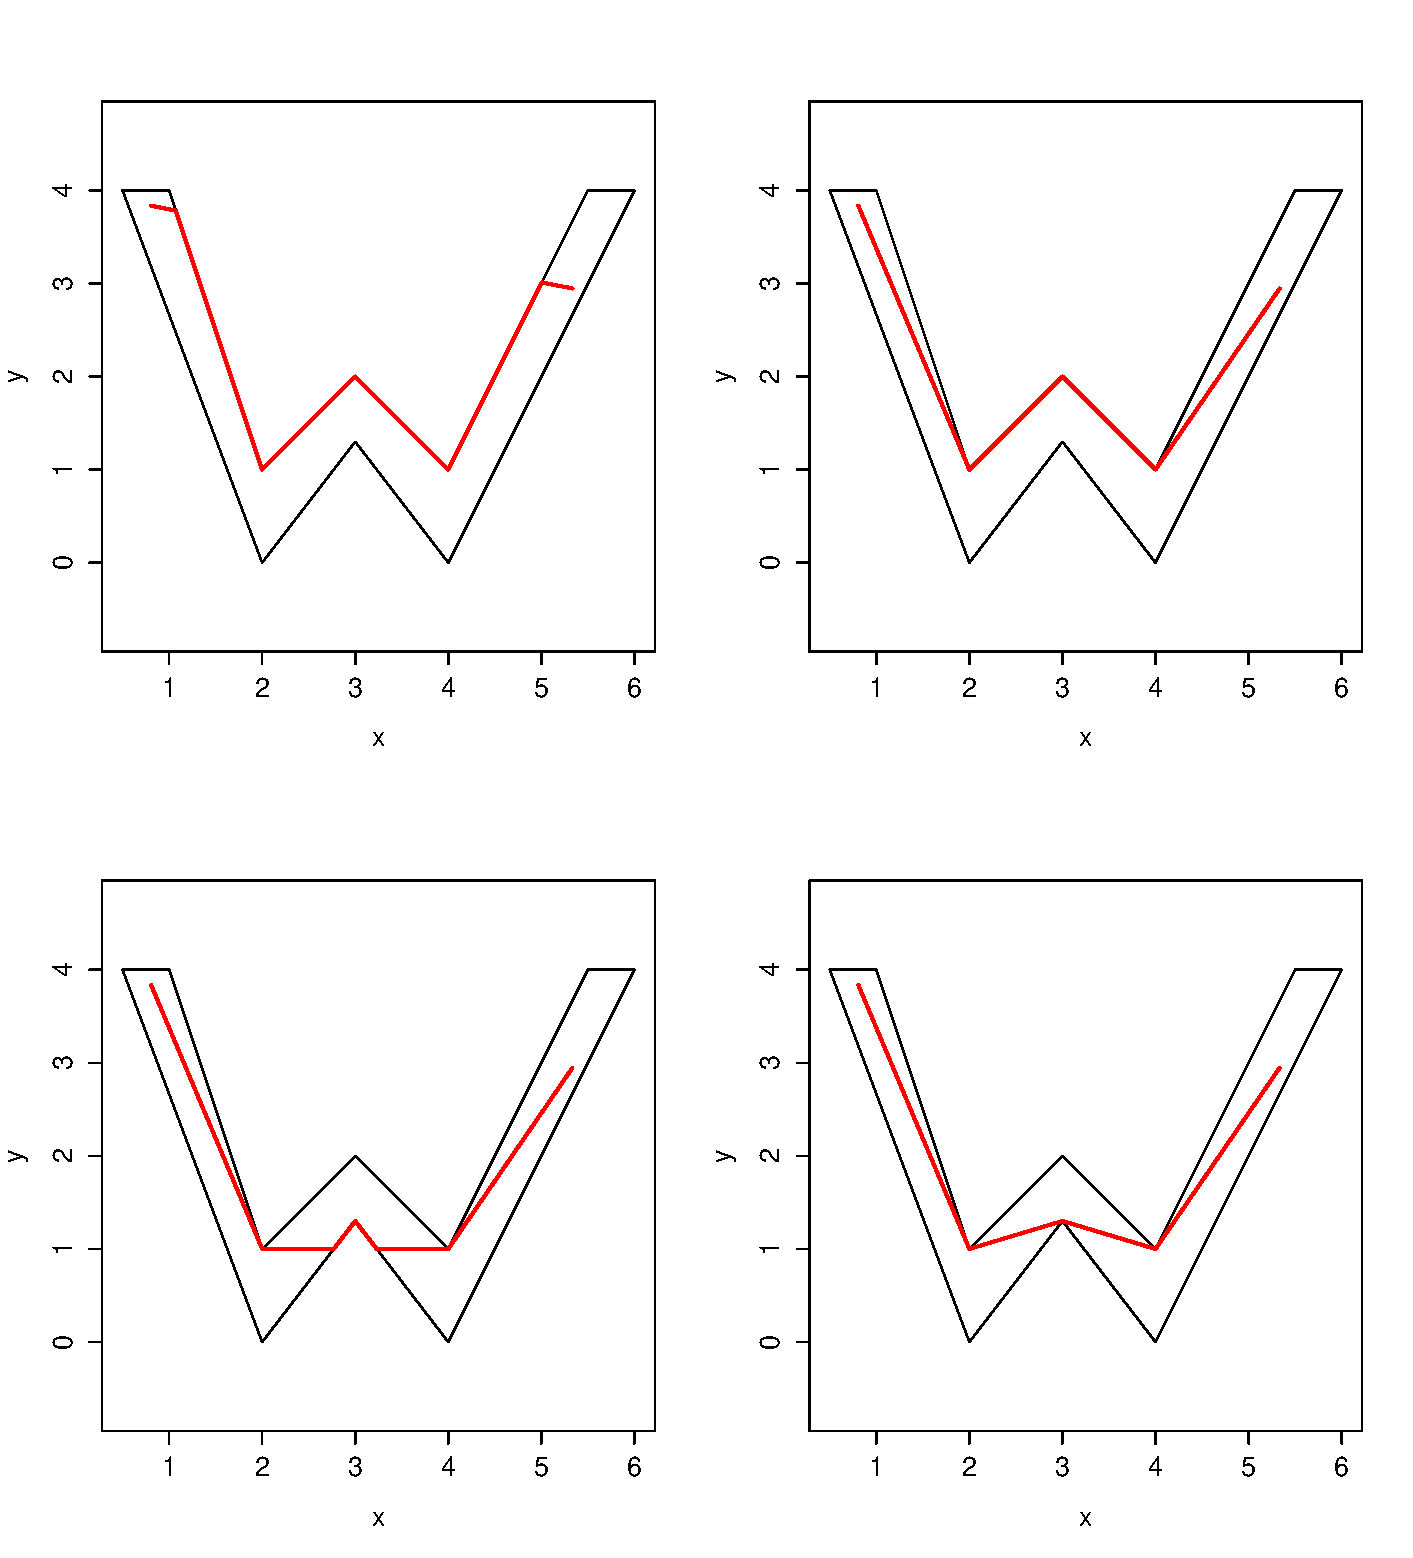
\includegraphics[width=2.75in]{figs/doubleyah-example.pdf}\\
\end{frame}



\subsection{Simulation Results}

\begin{frame}
	\frametitle{Ramsay simulations (low noise)}
            \centering
              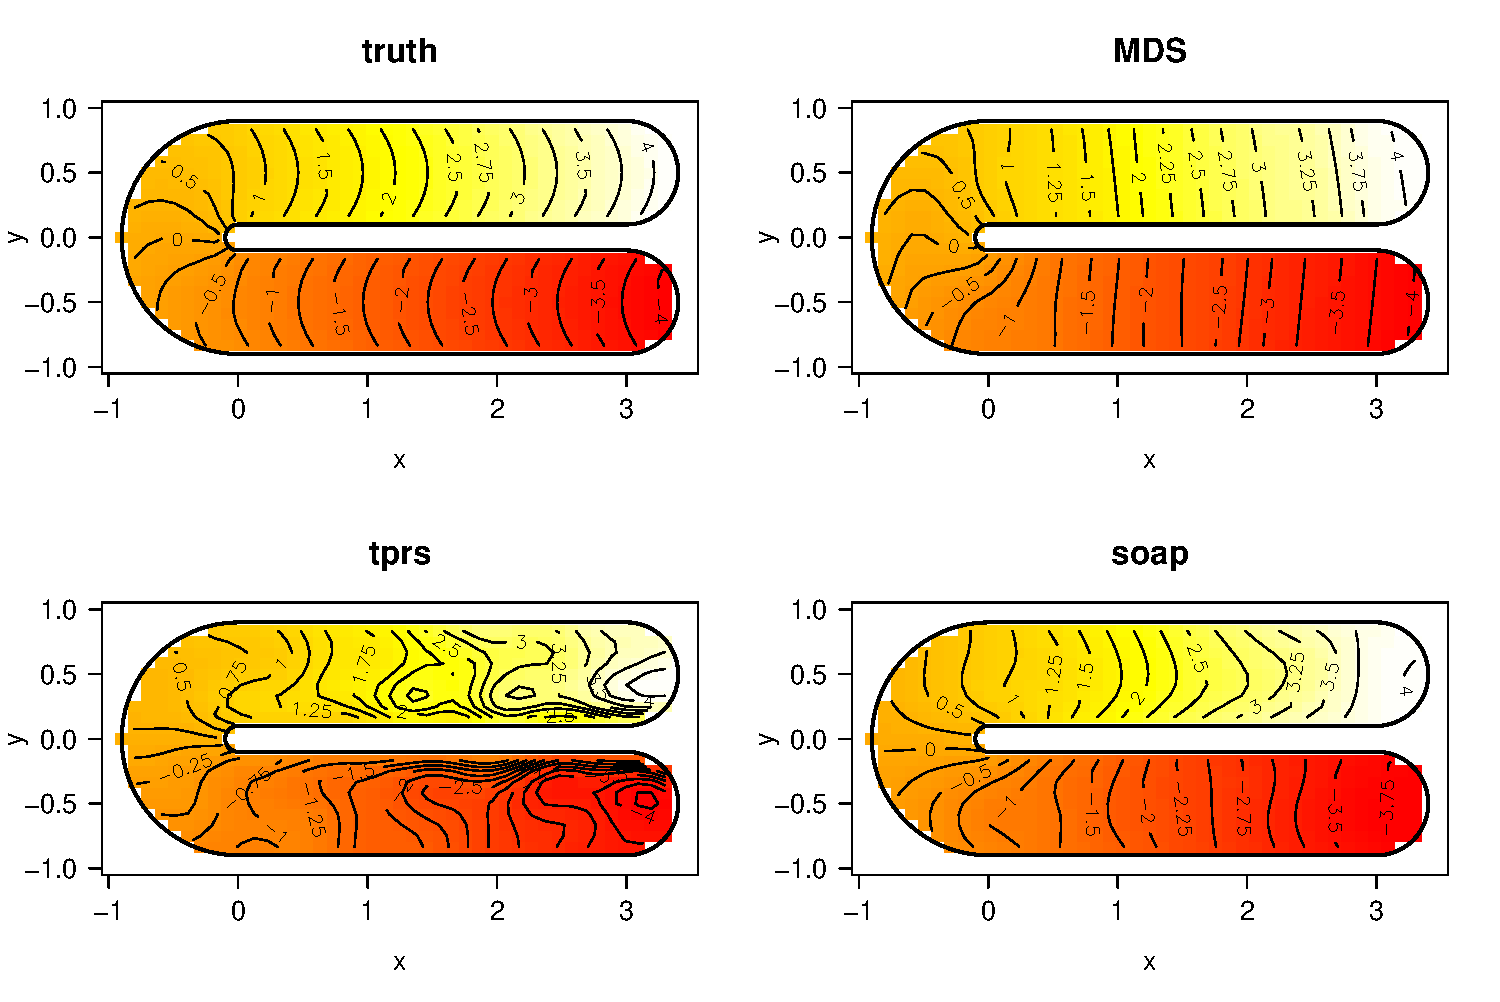
\includegraphics[width=4in]{figs/ramsay-low.pdf}\\
\end{frame}

\begin{frame}
	\frametitle{Ramsay simulations (high noise)}
            \centering
              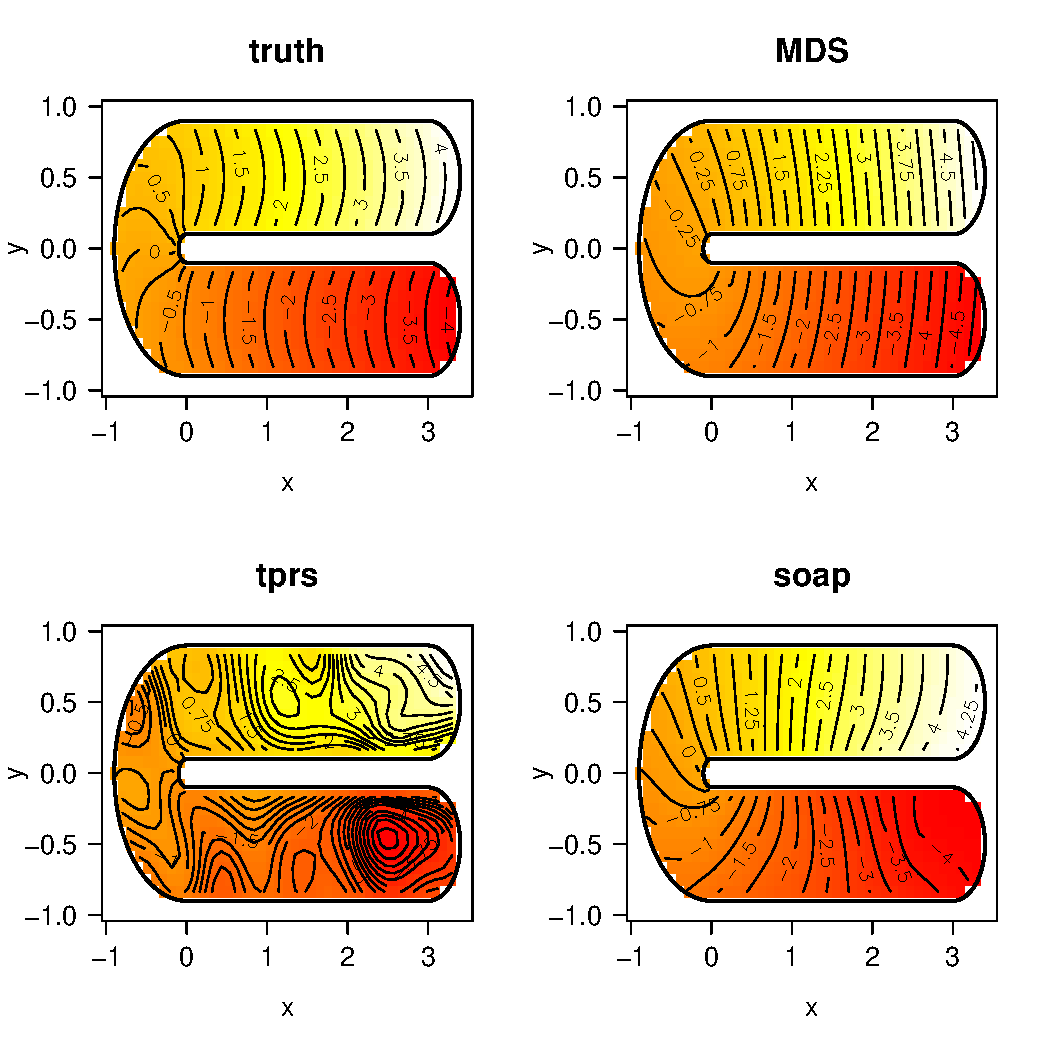
\includegraphics[width=4in]{figs/ramsay-high.pdf}\\
\end{frame}

\begin{frame}
	\frametitle{A different domain}
            \centering
              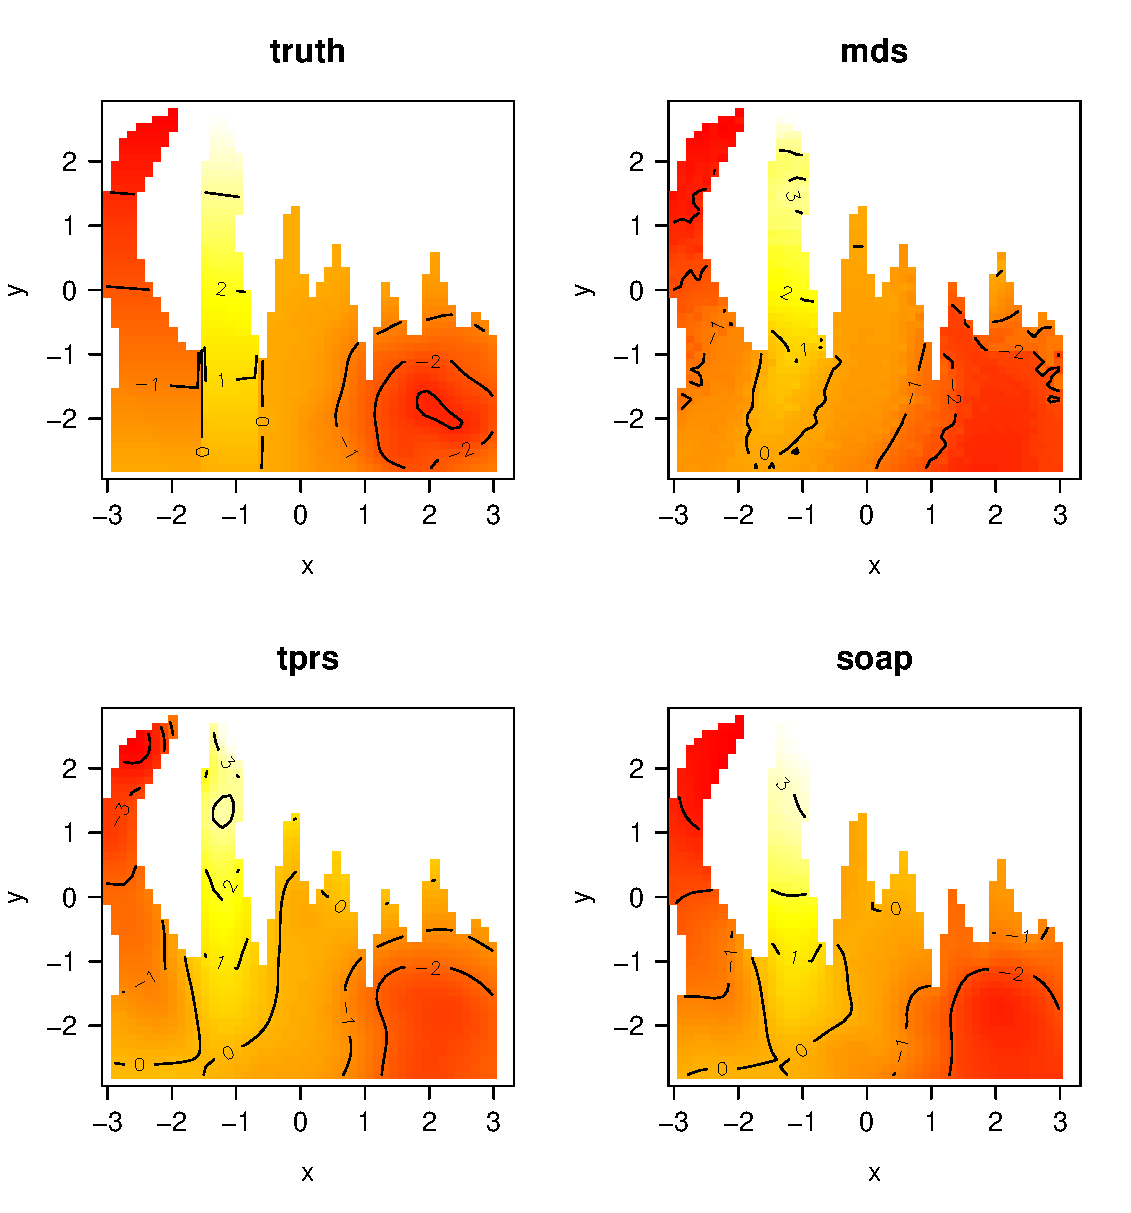
\includegraphics[width=3.25in]{figs/wt2-real.pdf}\\
\end{frame}

\section{Conclusions}

\begin{frame}
	\frametitle{Conclusions}
       \bi
         \item Seems that the S-C transform does not have much utility.
         \item MDS shows more promise, easier to transfer to higher dimensions.
         \item MDS does not impose strict boundary conditions so leakage still possible.
         \item After initial ``transform'' calculation, both methods only use the same computational time as a thin plate regression spline. (Soap is expensive.)
        \ei
\end{frame}

\begin{frame}
	\frametitle{Further work}
       \bi
         \item Real data!
         \item Implement insertion of new points using method of Gower (1968).
         \item Current within-area distance algorithm is pure R, very slow. Need to re-write in C/Fortran.
         \item Pushing the data into more dimensions might be useful to separate points.  
        \ei
\end{frame}




\begin{frame}
	\frametitle{References}
       \bi
         \item S.N. Wood, M.V. Bravington, and S.L. Hedley. \emph{Soap film smoothing. JRSSB, 2008}
         \item H. Wang and M.G. Ranalli. \emph{Low-rank smoothing splines on complicated domains. Biometrics, 2007}
         \item T.A. Driscoll and L.N. Trefethen. \emph{Schwarz-Christoffel Mapping. Cambridge, 2002}
         \item T. Ramsay. \emph{Spline smoothing over difficult regions. JRSSB, 2001}
         \item P.H.C. Eilers. \emph{P-spline smoothing on difficult domains. University of Munich seminar, 2006}
	\item C. Chatfield and A.J. Colins. \emph{Introduction to multivariate analysis. CRC, 1980}
	\item J.C. Gower. \emph{Adding a point to vector diagrams in multivariate analysis. Biometrika, 1968.}
        \ei
        Slides available at \url{http://people.bath.ac.uk/dlm27}
\end{frame}


\end{document}
